\chapter{Background} \label{chap:background}
%%%%%%%%%%%%%%%%%%%%%%%%%%%%%%%%%%%%%%%%%%%%
\section{RGB-D Cameras}
%%%%%%%%%%%%%%%%%%%%%%%%%%%%%%%%%%%%%%%%%%%%

%----------------------------------------------
\subsection{General}
%----------------------------------------------
RGB-D cameras have been widely used in many modern computer vision areas, for example 3D reconstruction~\cite{newcombe2011kinectfusion}, visual odometry and mapping on quadrocopter~\cite{huang2017visual} and visual SLAM algorithms~\cite{engelhard2011real}. 
A RGB-D camera returns a color image which is usually in RGB color space, and a depth map, every pixel of which reflects the real-world distance between the camera and the corresponding position of the pixel.
Depending on the technologies used to measure the depth information, the RGB-D camera can be divided to passive and active~\cite{kerl2012msc}.

The so called passive RGBD-camera usually contains two RGB cameras with a known translation between them.
After taking one picture for each, the features in two pictures are matched and then the triangulation is applied to obtain the depth.
An illustration is shown in Fig.~\ref{fig:rgbd_camera_passive}.

Active technologies usually emit lights to the environment so it has the capability of acquiring depth images in a totally dark indoor scenario.
They can be furthered categorized as time of flight (ToF) or structured light approaches.

A ToF camera calculates the depth in each pixel by measuring the delay between the emission and the reflected time.
ToF cameras typically emit either pulsed light or modulated light.
The Microsoft Kinect 2.0 and IFM Efector are two examples of the ToF camera.

The RGB-D cameras with the structured light use a projector for a known pattern. 
Since the transformation between the camera the projector is pre-given, a camera observes the projected pattern and then triangulates to calculate the depth (Fig.~\ref{fig:rgbd_camera_active}).
The ASUS Xtion Pro Live, Intel RealSense R200 and Ensenso are several well-known cameras using structured lights.
It should be noted that many active stereo cameras project infrared (IR) lights. 
Due to the fact that sun is a source of infrared lights, the usage of these cameras is limited to the indoor environment.


\begin{figure}[!htbp]
\centering
\subfigure[Passive stereo]{\label{fig:rgbd_camera_passive} 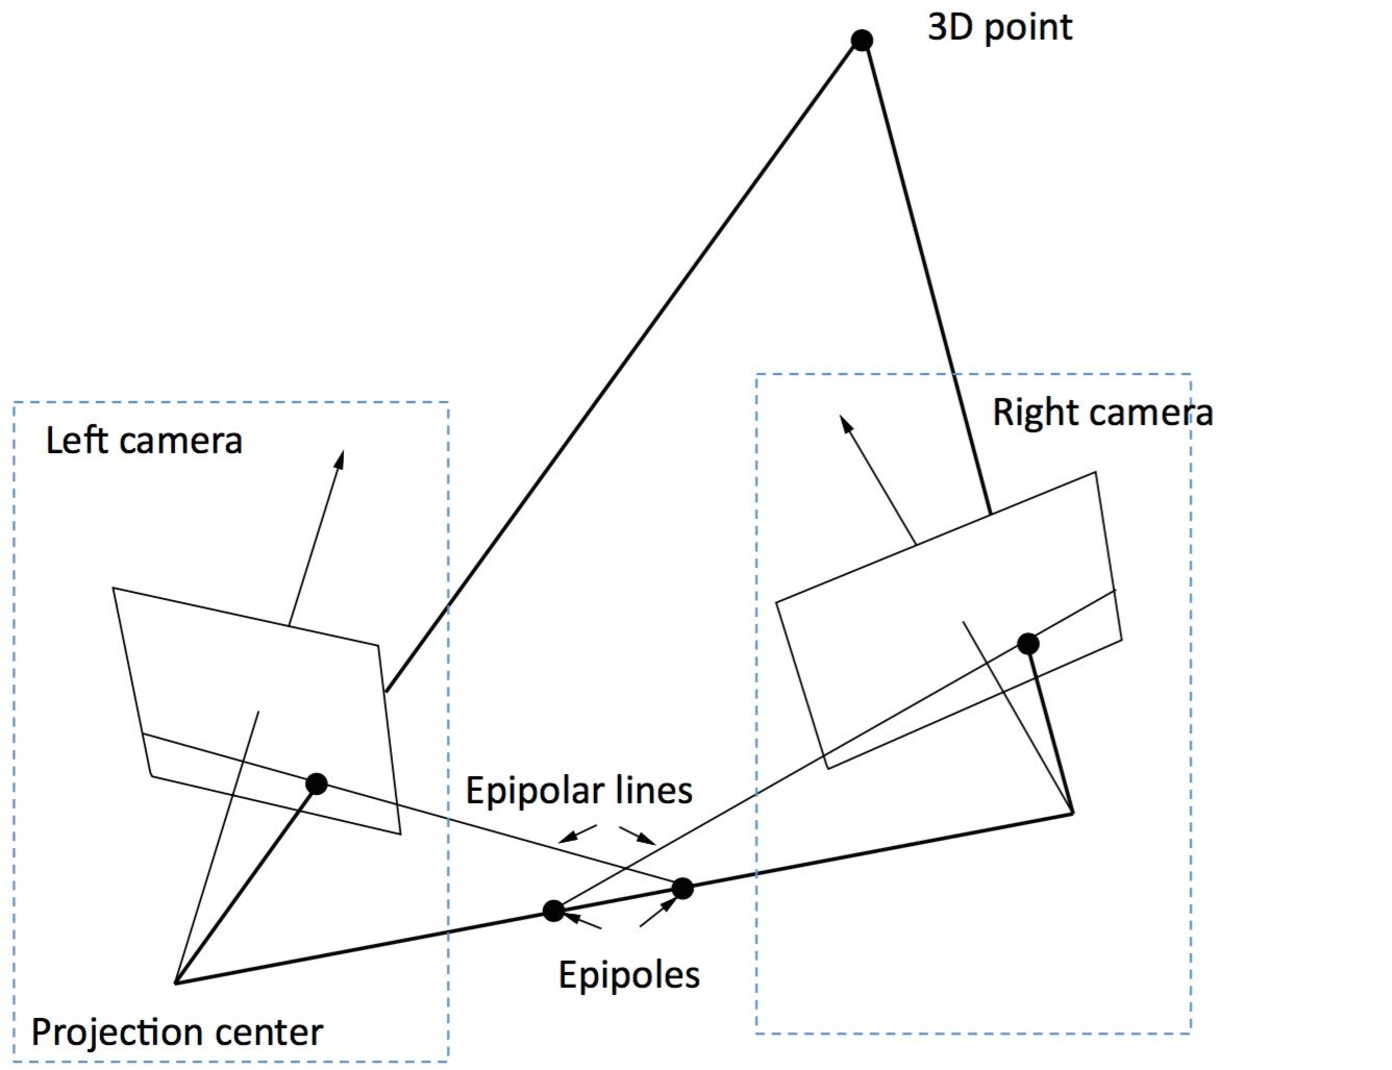
\includegraphics[width=0.40\linewidth]{figures/camera_passive.pdf}}
\subfigure[Active stereo]{\label{fig:rgbd_camera_active} 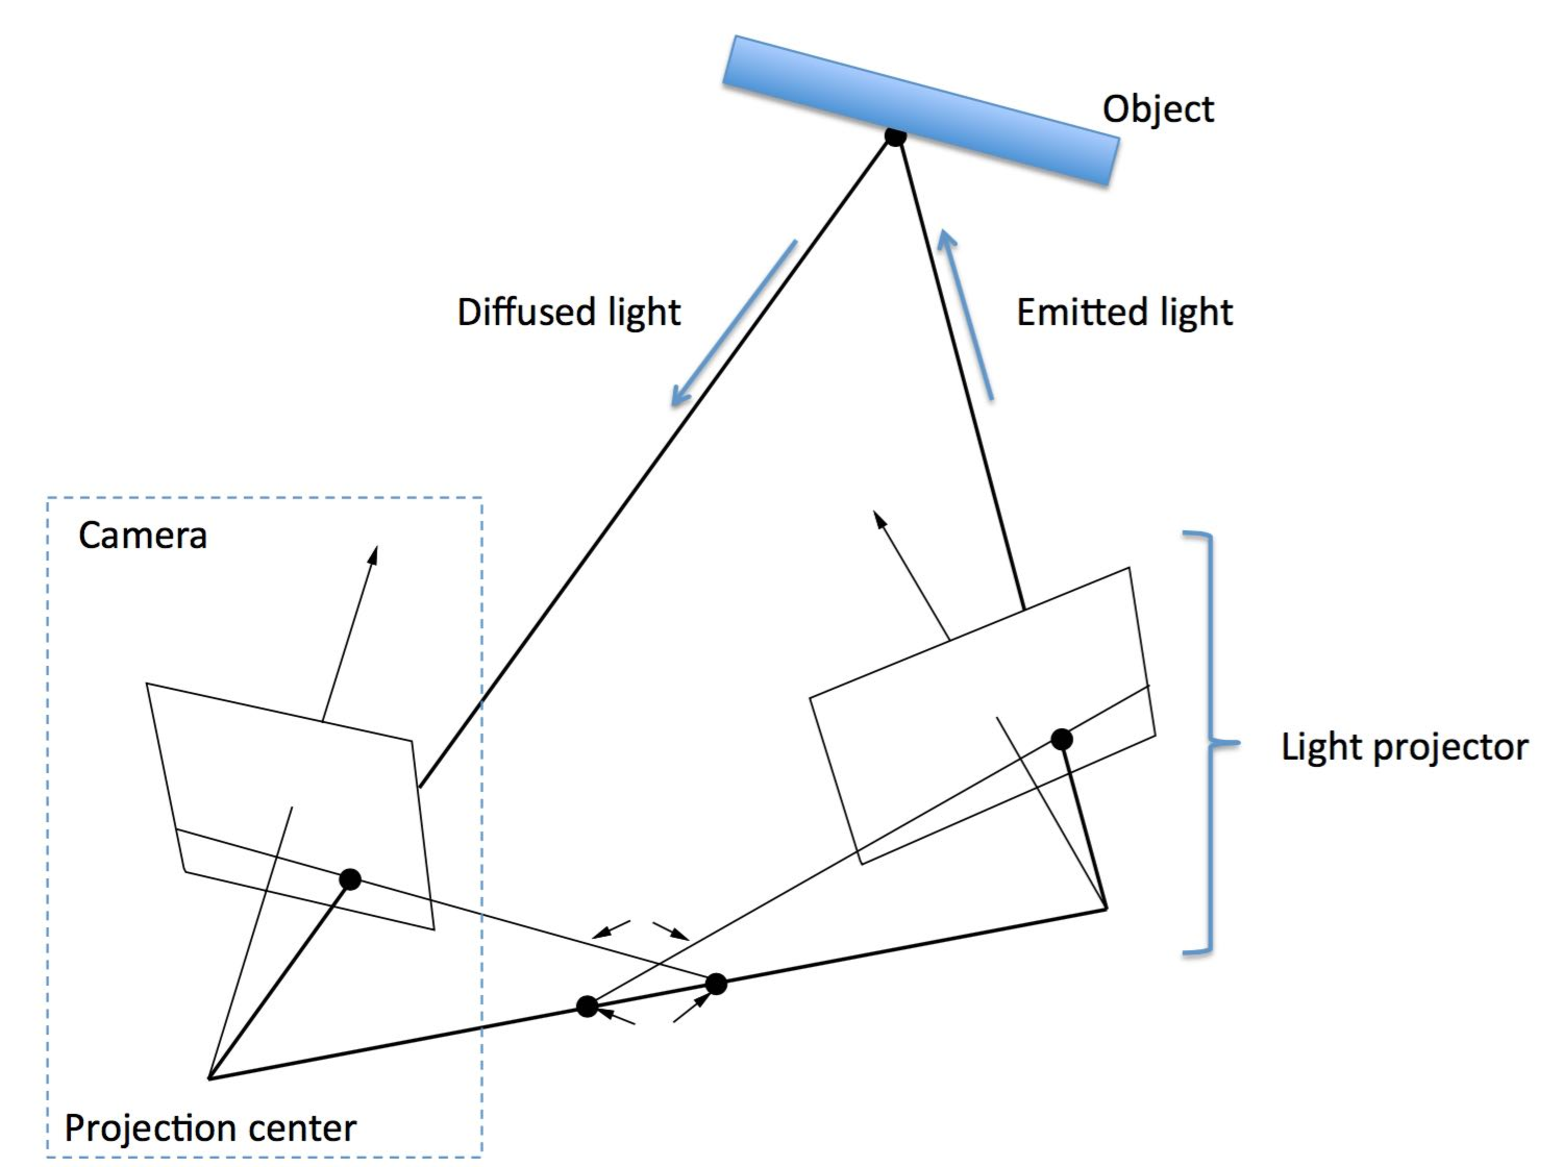
\includegraphics[width=0.45\linewidth]{figures/camera_active.pdf}}
\caption{Illustrations for the principle of passive and active stereo. Image courtesy of~\cite{horaud2013tutorial}.}
\label{fig:rgbd_camera}
\end{figure}


%%%%%%%%%%%%%%%%%%%%%%%%%%%%%%%%%%%%%%%%%%%%
\subsection{ASUS Xtion PRO LIVE}
%%%%%%%%%%%%%%%%%%%%%%%%%%%%%%%%%%%%%%%%%%%%

\begin{figure}[!ht]
\centering
\subfigure[Camera structure~\cite{asus}]{\label{fig:asus_structure} 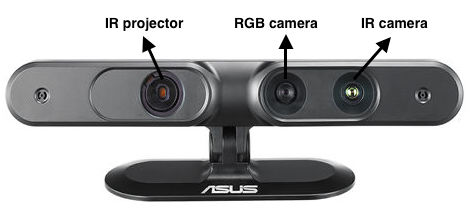
\includegraphics[width=0.4\linewidth]{figures/asus.jpg}}\\
\subfigure[RGB image]{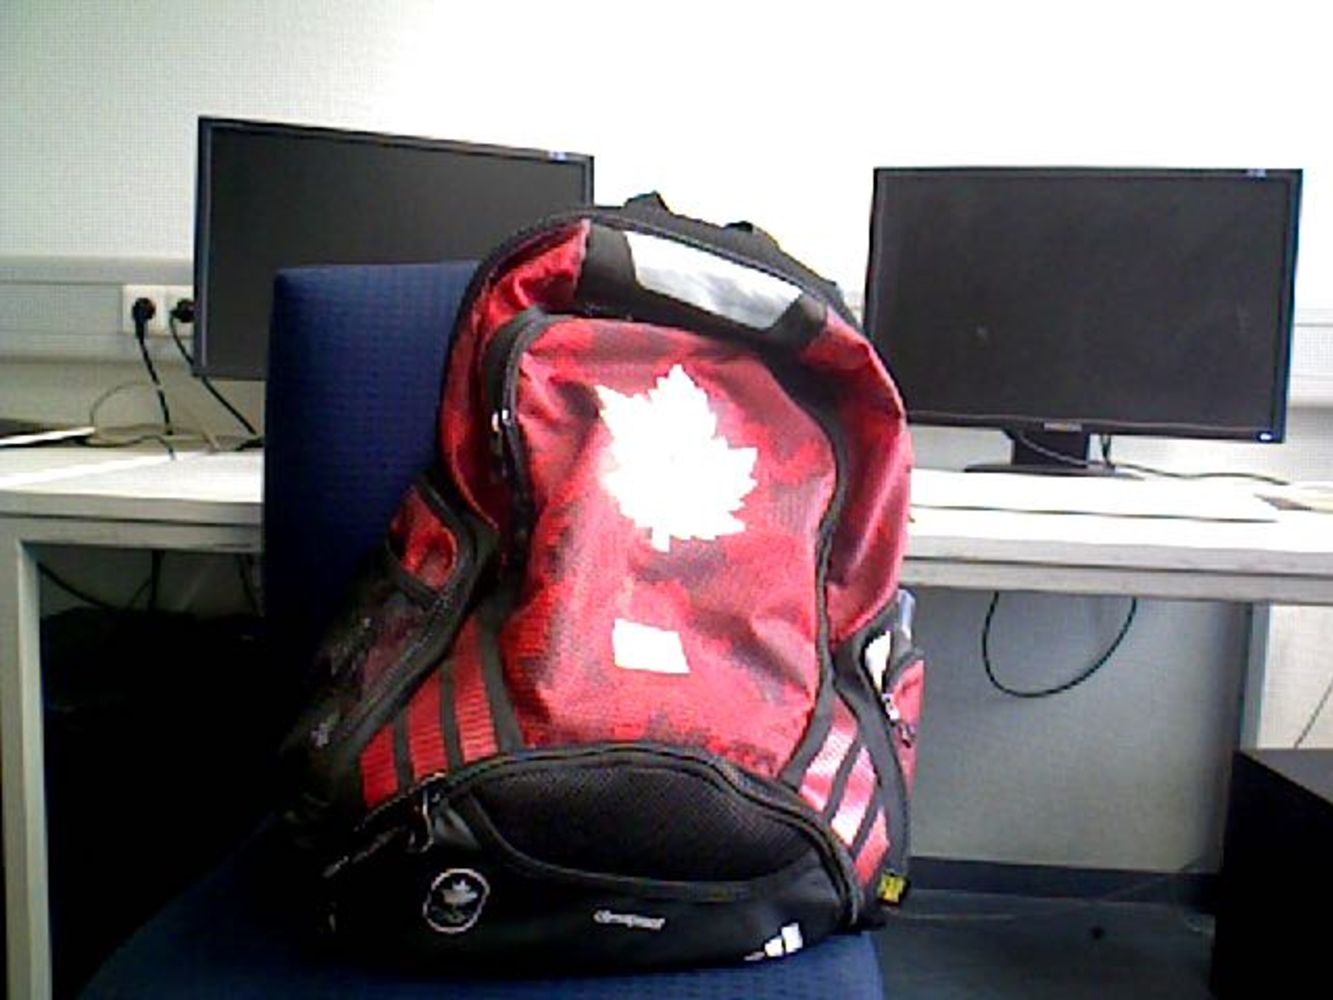
\includegraphics[width=0.4\linewidth]{figures/scene_rgb.pdf}}
\subfigure[Depth image]{ 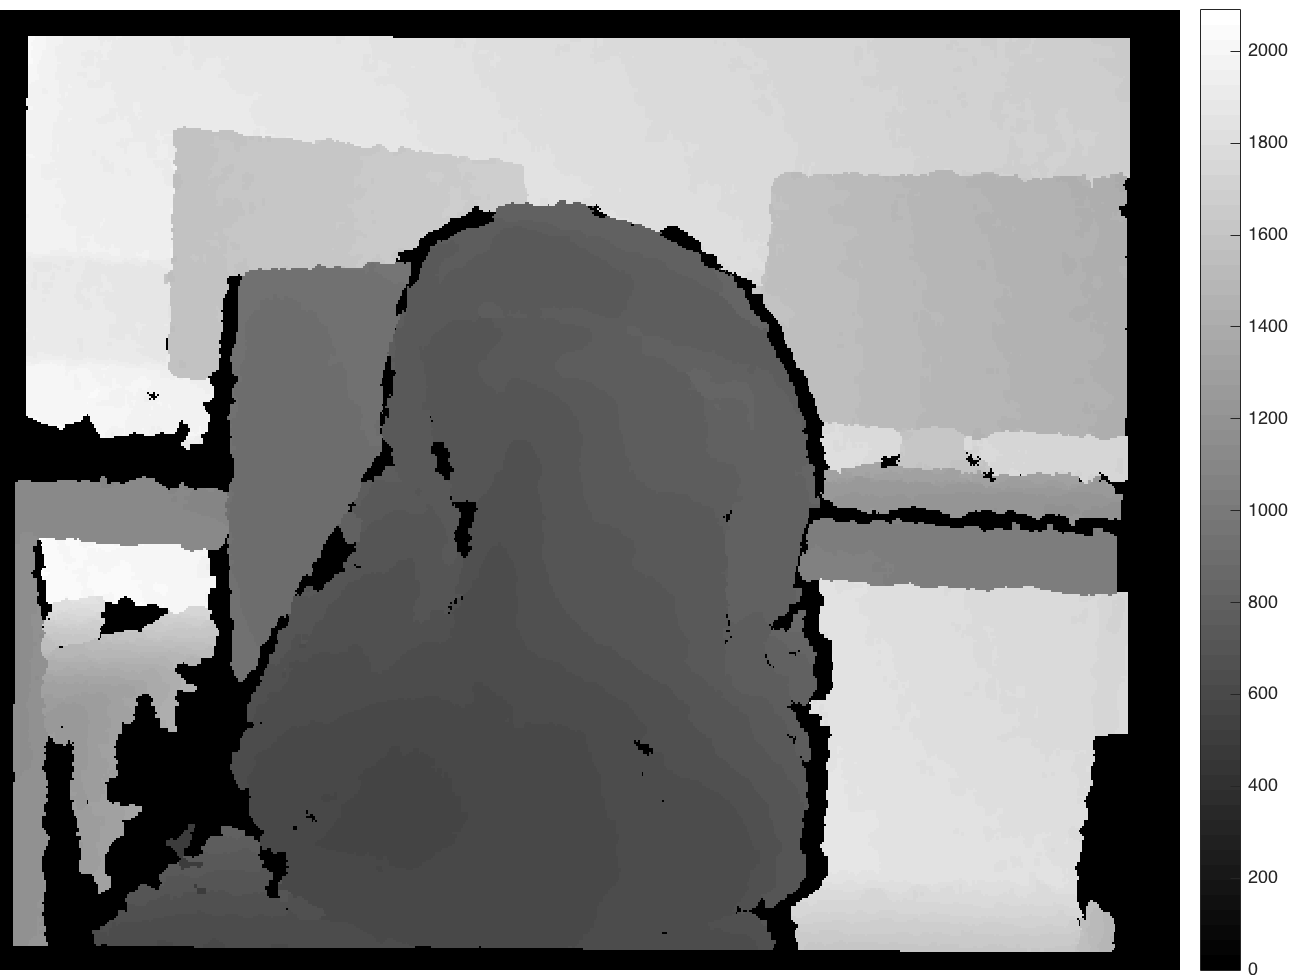
\includegraphics[width=0.4\linewidth]{figures/scene_depth.png}}
\caption{The structure of ASUS Xtion Pro Live and the RGB and depth images of an indoor scene acquired by it.}
\label{fig:asus_illustration}
\end{figure}
The ASUS Xtion Pro Live camera has two cameras and an IR projector as shown in Fig.~\ref{fig:asus_structure}.
According to the official website~\cite{asus}, it provides the RGB image with the maximum resolution of $1280\times1024$, while the depth can be alternated either VGA resolution ($640\times480$ with 30fps) or QVGA ($320\times240$ with 60fps). 
Its depth is reported to range from 0.8 to 3.5m, but we found in the experiments that the blind area was less and merely around 0.5m.  
Xtion Pro Live has been used throughout our experiments and we choose different configurations depending on the applications.
When the depth super-resolution is required, the RGB images have the resolution of $1280\times1024$, otherwise we keep the same RGB resolution as the depth ($640\times480$).

%%%%%%%%%%%%%%%%%%%%%%%%%%%%%%%%%%%%%%%%%%%%
\section{Shape from Shading \& Photometric Stereo}

The well-known shape from shading (SFS) problem was first introduced by Horn~\cite{horn1970shape} in 1970 and then a large amount of literature flooded in to develop the field.
The idea of SFS is, knowing the light source position, one can estimate the shape or the surface of an object from one single grayscale image.
This inverse problem is highly ill-posed, as illustrated in Fig.~\ref{fig:paint}.


\begin{figure}[!ht]
\centering
\subfigure[An image]{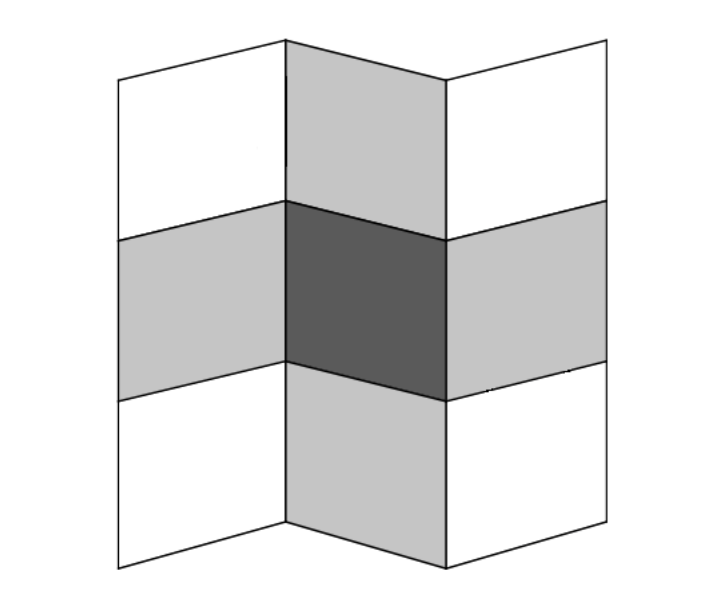
\includegraphics[width=0.25\linewidth]{figures/paint.png}}
\subfigure[A possible explanation~\cite{barron2015shape}]{ 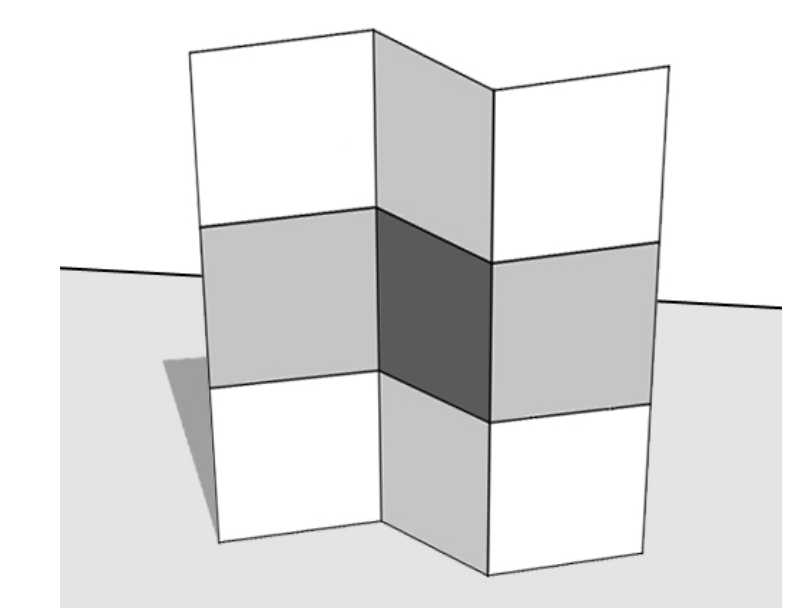
\includegraphics[width=0.3\linewidth]{figures/paint0.png}}\\
\subfigure[painter's explanation]{
\includegraphics[width=0.2\linewidth]{figures/paint1.png}}
\subfigure[sculptor's explanation]{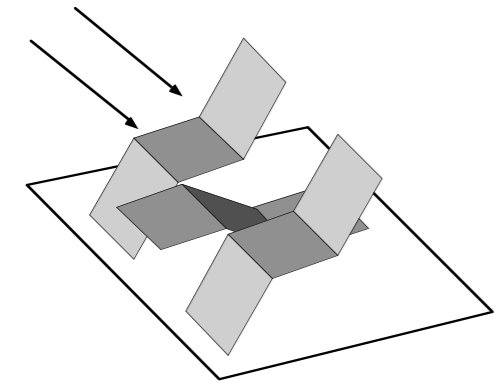
\includegraphics[width=0.3\linewidth]{figures/paint2.png}}
\subfigure[Lighting designer's explanation]{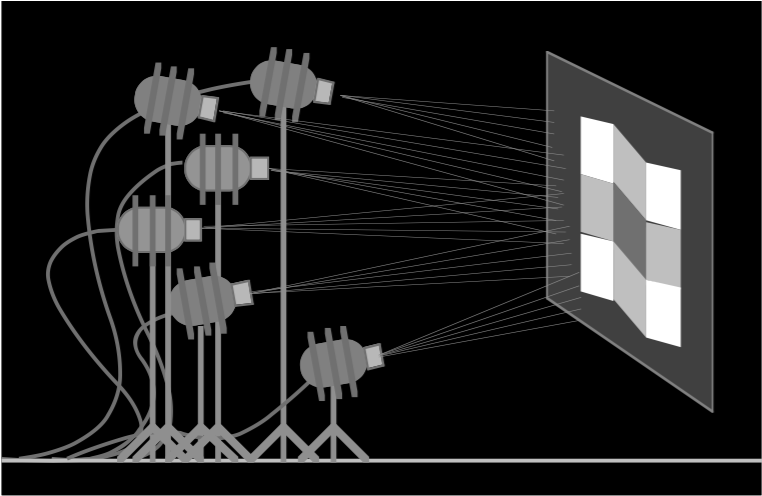
\includegraphics[width=0.3\linewidth]{figures/paint3.png}}
\caption{Various explanations for a twice-bent surface. Images are from~\cite{adelson1996perception}}
\label{fig:paint}
\end{figure}


From the mathematical perspective, the luminance can be separated as follows:
\begin{equation}\label{eq:sfs_equation}
    I = \rho S
\end{equation}
where $I$ is an intensity image, $\rho$ is the reflectance (albedo) of the surface, and the $S$ is the shading image. 
An example of such an image decomposition is shown in Fig.~\ref{fig:shading}.
%&&&&&&&&&&&&&&&&&&&&&&&&&
\begin{figure}[!htbp]
\centering
\setlength{\tabcolsep}{0.1em} % column spacing
 {\renewcommand{\arraystretch}{0.6}% row spacing
\begin{tabular}{c c c c c}
   
\includegraphics[height = 0.16\linewidth]{figures/panther_rgb.pdf} \hspace{0.05cm}   &
   \multirow{-10}{*}{\parbox[t]{3.5mm}{=}}  & 
   
\includegraphics[height = 0.16\linewidth]{figures/panther_rho.pdf} &
    \multirow{-10}{*}{\parbox[t]{3.5mm}{$\times$}}  & 
   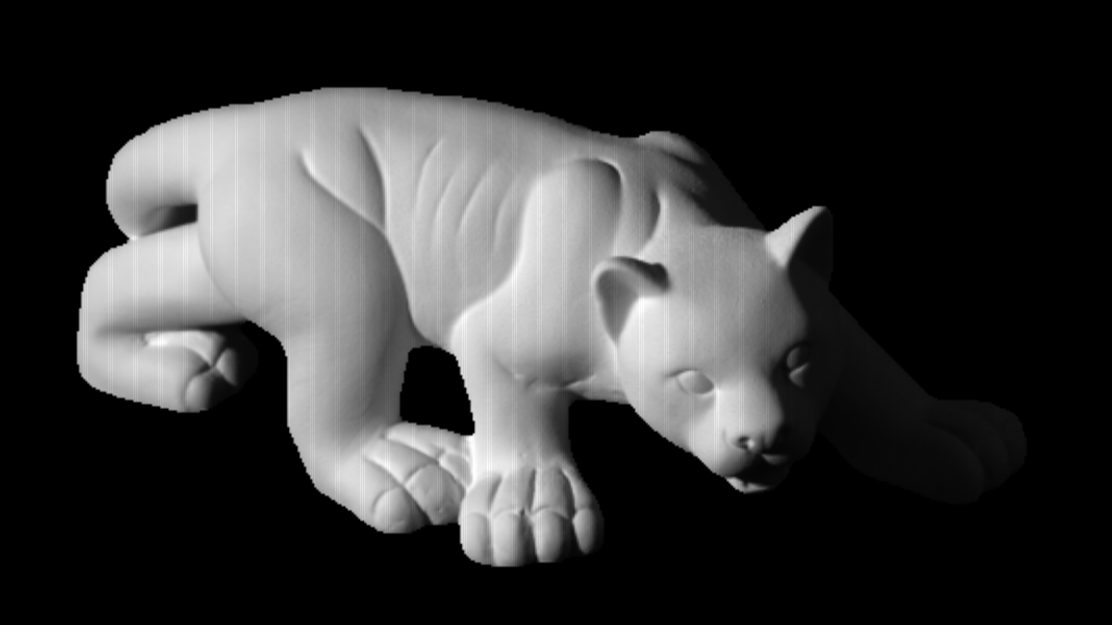
\includegraphics[height = 0.16\linewidth]{figures/panther_shade.pdf} \\
      {I} &{} &{$\rho$} & {}& {$S$}            
 \end{tabular}}
\caption{The decomposition of a color toy panther. Images are from MIT intrinsic images dataset~\cite{grosse2009ground}.}
\label{fig:shading}
\end{figure}
%&&&&&&&&&&&&&&&&&&&&&&&&&

SFS approches assume the observed object follows the Lambert's cosine law~\cite{klett1760ih}, based on which the Eq.~\ref{eq:sfs_equation} can be reformulated to the Lambertian reflectance model:
\begin{equation}\label{eq:lambertian_model}
    I = \rho \; \mathbf{l}^\top \mathbf{n}
\end{equation}
where we can notice that the shading $S$ is the inner product of the light direction and the surface normal.
Thus, the task of SFS is to retrieve the shape (surface normal) from the shading based on the Lambertian reflectance model.
Moreover, many state-of-the-art shape or depth refinement methods used an extension of Lambertian model called spherical harmonics (SH) \cite{basri2003lambertian, ramamoorthi2001relationship} which can represent the illumination more realistically. 
It has been shown that the first-order SH model (Eq.~\ref{eq:sh_model}) can account for $87.5\%$ of real world light so we applied it throughout the whole thesis:
\begin{equation}\label{eq:sh_model}
    I = \rho \; (\mathbf{l}^\top \mathbf{n} + \varphi)
\end{equation}
where $\varphi$ can be understood as the ambient light parameter.

The goal of SFS is to estimate the shape or the surface of object, which is represented by the surface normal $\mathbf{n}$.
Two camera projection models are usually used for modelling the surface normal: orthographic and perspective projection.
To derive $\mathbf{n}$ using orthographic projection, we consider projection along the $z$-axis\cite{hartley2003multiple}.
Hence, A 3D point $P = (x,y,z)$ is mapped to the image point $p = (x,y)$.
It should be noted that the depth $z$ depends on the coordinate $x$ and $y$.
And we know the surface normal is orthogonal to the tangent plane in $(x,y)$, which can be written as:
\begin{equation}
    \mathbf{n}(P) \propto \; \partial_x P \times \partial_y P 
    = \begin{pmatrix} 1 \\ 0 \\ z_x\end{pmatrix}
    \times \begin{pmatrix} 0 \\ 1 \\ z_y\end{pmatrix}
    = -\begin{pmatrix} z_x \\ z_y \\ -1\end{pmatrix}
\end{equation}
After normalizing and choosing the outward direction, we acquire the unit-length surface normal with orthographic projection:
\begin{equation}
    \mathbf{n}_{ortho} = \frac{1}{\sqrt{|\nabla z| + 1}} \begin{pmatrix} \nabla z \\ -1\end{pmatrix}
\end{equation}
For the more realistic perspective model, the 3D point $P$ now becomes $\begin{pmatrix} (x - x_0)/f \\ (y - y_0)/f\\ z\end{pmatrix}$ and the corresponding normal is:
%$$$$$$$$$$$$$$$$
\begin{equation}\label{eq:ratio_normal}
    \mathbf{n}_{perspect} =
    \frac{1}{d}
     \begin{pmatrix}
         f\tilde{z}_x\\
         f\tilde{z}_y\\
         -1 - (x-x_0)\tilde{z}_x - (y - y_0)\tilde{z}_y
     \end{pmatrix}
\end{equation}
%$$$$$$$$$$$$$$$$
where $\tilde{z} = \log{z}$, $f$ the focal length, $(x_0, y_0)$ the coordinates of principle points, and the normalizer $d =  \sqrt{(f\tilde{z}_x)^2 + (f\tilde{z}_y)^2 + (-1 - (x-x_0)\tilde{z}_x - (y - y_0)\tilde{z}_y)^2}$.

From the definition of the surface normal, we can notice the SFS is an ambiguous problem. 
Even when the lighting and the albedo are known in Eq.~\ref{eq:lambertian_model}, the inverse problem is ill-posed because the normal has 2 degrees of freedom. 
As we can see from Fig.~\ref{fig:paint}, the solution of SFS is ambiguous.
Horn and Brooks~\cite{horn1986variational} proposed the so-called integrability constraint $z_{xy} = z_{yx}$, which was the first constraint imposed on surface normal to make the SFS problem well-posed. 
Frankot and Chellapa~\cite{frankot1988method} projected a non-integrable surface to the subspace spanning the valid smooth surface.


Provided we have several images from the same view but with different illuminations, Eq.~\ref{eq:sfs_equation} can be modelled as:
\begin{equation}\label{eq:ps_equation}
    \mathbf{I = BL}
\end{equation}
Assuming there are $n \geqslant 3$ images from various illumination conditions, with $m$ pixels in each image, $\mathbf{I}\in \mathbb{R}^{m\times n}$ is the stack of all the intensity images and each column of $\mathbf{I}$ represents a vectorized image from a lighting condition.
 $\mathbf{B}\in\mathbb{R}^{m\times3}$ corresponds to $\rho \boldsymbol{\cdot} \mathbf{n}^\top$ and $\mathbf{L}\in\mathbb{R}^{3\times n}$ represents $ n$ various lightings.
If the illuminations are known, we call this problem \emph{calibrated} photometric stereo (PS), which was first introduced by Woodham~\cite{woodham1980photometric} in 1980. The problem is over-constrained so the surface normals can be estimated using a simple least squares. 
Some regions may sometimes suffer from the shadows for a certain illumination, so Forsythe and Ponce~\cite{forsyth2003modern} formed a diagonal matrix to eliminate all those shadow points.
Another interesting example of calibrated PS was proposed by Hern{\'a}ndez \emph{et al.}~\cite{hernandez2011overcoming}.
They controlled red, green, and blue lights from three directions and acquired the shape from only one color image, every channel of which was treated as a separate intensity image.   
This was one of the inspiration of our first proposed method RGB ratio model, which will be detailed in chapter~\ref{chap:methodology}.

However, the different lightings are not always controlled or given, then we call this kind of problem \emph{uncalibrated} photometric stereo. 
Hayakawa~\cite{hayakawa1994photometric} found that the surface normals and the albedo could be recovered with a $3\times3$ linear transformation using singular value decomposition. Yuille and Snow~\cite{yuille1997shape} further reduced the ambiguity to a gerenalized bas-relief (GBR) ambiguity by adding the integrability constraint. Now Eq.~\ref{eq:ps_equation} can be represented as
\begin{equation}\label{eq:ps_gbr}
    \mathbf{I} = \mathbf{B}\mathbf{A}^{-1}\mathbf{A}\mathbf{L}    
\end{equation}
where $\mathbf{A}$ is the GBR matrix:
\begin{equation}
    \mathbf{A} = 
    \begin{pmatrix}
        1& 0 & 0\\
        0& 1 & 0\\
        \mu & \nu & \lambda
    \end{pmatrix}
\end{equation}

There is a large amount of research work trying to solve the GBR ambiguity in uncalibrated PS.
Alldrin \emph{et al.}~\cite{alldrin2007resolving} used the prior emphasizing that the albedo distribution should have a low entropy, to resolve the ambiguity.
Favaro and Papadhimitri~\cite{papadhimitri2014closed} eliminated the ambiguity by exploiting the spatial maximum points of the inner product between the normals and the lights.
They also found out the solution is unique when the normal is constructed under the perspecitve projection instead of the orthographic projection~\cite{papadhimitri2013new}.
Qu\'{e}au \emph{et al.}~\cite{queau2015solving} estimated the GBR parameters by imposing the total variation norm.

In terms of depth, the GBR ambiguity is equivalent to the equation~\cite{belhumeur1999bas}:
\begin{equation}
    z(x,y) = \lambda z(x,y) + \mu x + \nu y
\end{equation}
Based on the equation, we find out that the GBR ambiguity still exists for the task of depth estimation.
However, since the rough depth will be given as the input from RGB-D camera, the GBR ambiguity problem encountered by uncalibrated PS is resolved automatically.
%Two examples about GBR ambiguity can be seen in Fig.~\ref{fig:ps_comp_syn} and~\ref{fig:ps_comp}.
Therefore, we will discuss some state-of-the-art depth refinement approaches.

 

\section{Depth and Shape Refinement}
%%%%%%%%%%%%%%%%%%%%%%%%%%%%%%%%%%%%%%%%%%%%

In recent years, there is a large amount of literature focusing on the depth or shape refinement based on either SFS (only use one single image) or PS (multiple images with different illuminations).
They are collectively called shading-based methods.
We will discuss these two streams respectively in the following.
%----------------------------------------------
\subsection{SFS-based methods}
%----------------------------------------------
Since SFS iteslf uses only one input image, it suffers from some intrinsic ambiguities that we have mentioned in the last section even when the light and the albedo are specified, so there will be more than one possible solution.
Now, although a rough depth map is given, the illumination and the albedo are unknown, so some regularization terms have to be imposed in order to acquire an exact solution from the inverse problem.

Han \emph{et al.}~\cite{han2013high} presented a framework which combines a global lighting model using the given color and depth with the help of SH model, with a local lighting model which varies spatially. 
The surface orientations should obey the integrability constraint on the smooth surface so they enforced the constraint by penalizing the curl of local neighborings.
However, the albedo in their method is assumed to be uniform.
To handle the multi-albedo objects, they had to apply another intrinsic image decomposition algorithm~\cite{barron2011high} and k-mean clustering to group the albedos into some areas with constant values inside.
Such framework is not only unrealistic but also very time-consuming so not able to be adapted to the real-world applications.

Yu \emph{et al.}~\cite{yu2013shading} iteratively update SH lighting and the albedo using the initial depth and the refined the shape with the estimated lighting and the relative albedo. 
They performed mean-shift clustering to segment the input RGB image into small regions with uniform albedo, and then obtained the relative albedos among various segmented regions. 
To fill in the missing depth information, a constrained texture synthesis and patch-based repairing scheme was applied.
In constrast, we efficiently apply a basic image inpainting approach as the pre-processing and the results are also satisfactory.


Wu \emph{et al.}~\cite{wu2014real} extended their previous offline shading-based refinement work~\cite{wu2011shading} to online shape refinement with highly parallel scheme and the help of GPU. 
They first calculated the 2nd-order SH parameters with the assumption of uniform albedo, and then estimated the albedo by simply dividing RGB image with the shading term.
We will show in chapter~\ref{chap:methodology} that this process may lead to the severe albedo overfitting problem such that the albedo estimation is not correct.
The shape is then refined in real-time by finding the surface that minimizes the difference between the shading and intensity image gradients.
Thereafter, the coarse depth map was directly refined with smoothness and temporal constraint on the video by using a Gauss-Newton solver on GPU.

Kim \emph{et al.}~\cite{kim2015joint} used a joint energy to estimate the depth, albedo and the light with smoothness regularization terms.
An anisotropic Laplacian constraint on chromaticity was introduced for albedo and a local smoothness and bas-relief ambiguity similar to~\cite{barron2013intrinsic} constraints are imposed for depth.
Based on our testing implementation, it has turned out that the Laplacian on chromaticity of the image cannot provide satisfactory albedos for the small indoor environment.
What's more, it is a very tedious process to tune all the parameters for the constraints.

RGBD-Fusion method from Or-El \emph{et al.}~\cite{or2015rgbd} can also deal with natural illumination conditions and make the depth recovery task in real time under GPU. 
They imposed the constraints not only on the albedo and depth estimation but also pixel-wise ambient lighting.
Their method does not really converge because of their way of handling the nonlinearity.
This inspired us to propose a new RGB ratio model to eliminate the nonlinearity. 


Or-El's following work~\cite{or2016real} can deal with specular objects with the help of IR camera and a more complicated reflectance model than spherical harmonics. 
In constrast, our proposed multi-light method still uses a Lambertian diffused reflectance model but can handle the specularity.

From what we have discussed, SFS methods are often limited to the uniform or constant albedo. 
For the sake of handling multi-albedo cases, some SFS methods~\cite{han2013high, yu2013shading} adapted segmentation methods to divide the input image into some constant albedo part, but the real-world objects are usually with complex multi-albedo and small regions, which makes the segmentation not accurate or incorrect.  
Some other methods~\cite{wu2014real,kim2015joint,or2015rgbd,or2016real} try to add some piecewise smooth constraints on the albedo but never really acquired satisfactory outcome.
Therefore, SFS-based methods using only one single image have the difficulty to separate the albedo from the surface normal, which may lead to the wrong depth estimation.

%----------------------------------------------
\subsection{PS-based methods}
%----------------------------------------------
Another category of shading-based depth refinement is PS-based methods.
With the help of multiple images acquired from various illuminations, these approaches can resolve the ambiguities tolerated by SFS methods and have a better performance in the separation between the albedo and surface normal.

Haque \emph{et al.}~\cite{haque2014high} proposed a method to reconstruct the shape and refine the depth using an IR camera without the need of RGB camera.
However, similar to many other multi-view photometric reconstruction approaches~\cite{park2013multiview, queau2017dense}, they assumed the albedo is restricted to uniform and thus, it is not suitable to use it for multi-albedo objects.

Their follow-up work from Chatterjee and Govindu~\cite{chatterjee2015photometric} decomposed the input images under different illuminations with a standard photometric stereo manner.
They used an iterative reweighted method to approximate the Rank 3 radiometric brightness matrix, then factorize it into the corresponding lighting, albedo and surface normal. 
They can cope with the multi-albedo objects but still have to use the IR images instead of RGB images. 
In this case, at least one extra infrared light source is always required, while in our case only a cheap LED light or even just the flashlight on a phone is enough.
Moreover, since the IR camera in ASUS Xtion Pro Live is limited to the resolution $640\times 480$, while the RGB camera can reach $1280\times 1024$, their approach can not perform depth super-resolution task like our multi-light method.

Wu \emph{et al.}~\cite{wu2011high} used second-order spherical harmonics to model general illumination and use the shading constraint to help improve the object reconstruction.
this method is extended to~\cite{wu2011shading} whose results are furthered improved by integrating a weak temporal prior on lighting, albedo and the shape.


In this thesis, we propose two shape refinement methods based on uncalibrated photometric stereo.
Similar to~\cite{hernandez2011overcoming}, we firstly used  red, green and blue LEDs for the active illuminations so we can treat  every channel of the obtained color image as an intensity image with light from a different direction.
Another proposed method needs only one white LED. 
With the RGB-D camera's angle of view fixed, we manually move the LED lights while the images are being taken.
Moreover, the shading-based method have never been applied for the depth map super-resolution before.
We successfully adapt our methods to depth super-resolution and achieved very pleasing outcomes. 
%%%%%%%%%%%%%%%%%%%%%%%%%%%%%%%%%%%%%%%%%%%%
